% Options for packages loaded elsewhere
\PassOptionsToPackage{unicode}{hyperref}
\PassOptionsToPackage{hyphens}{url}
%
\documentclass[
]{report}
\usepackage{amsmath,amssymb}
\usepackage{iftex}
\ifPDFTeX
  \usepackage[T1]{fontenc}
  \usepackage[utf8]{inputenc}
  \usepackage{textcomp} % provide euro and other symbols
\else % if luatex or xetex
  \usepackage{unicode-math} % this also loads fontspec
  \defaultfontfeatures{Scale=MatchLowercase}
  \defaultfontfeatures[\rmfamily]{Ligatures=TeX,Scale=1}
\fi
\usepackage{lmodern}
\ifPDFTeX\else
  % xetex/luatex font selection
\fi
% Use upquote if available, for straight quotes in verbatim environments
\IfFileExists{upquote.sty}{\usepackage{upquote}}{}
\IfFileExists{microtype.sty}{% use microtype if available
  \usepackage[]{microtype}
  \UseMicrotypeSet[protrusion]{basicmath} % disable protrusion for tt fonts
}{}
\makeatletter
\@ifundefined{KOMAClassName}{% if non-KOMA class
  \IfFileExists{parskip.sty}{%
    \usepackage{parskip}
  }{% else
    \setlength{\parindent}{0pt}
    \setlength{\parskip}{6pt plus 2pt minus 1pt}}
}{% if KOMA class
  \KOMAoptions{parskip=half}}
\makeatother
\usepackage{xcolor}
\usepackage{longtable,booktabs,array}
\usepackage{calc} % for calculating minipage widths
% Correct order of tables after \paragraph or \subparagraph
\usepackage{etoolbox}
\makeatletter
\patchcmd\longtable{\par}{\if@noskipsec\mbox{}\fi\par}{}{}
\makeatother
% Allow footnotes in longtable head/foot
\IfFileExists{footnotehyper.sty}{\usepackage{footnotehyper}}{\usepackage{footnote}}
\makesavenoteenv{longtable}
\usepackage{graphicx}
\makeatletter
\def\maxwidth{\ifdim\Gin@nat@width>\linewidth\linewidth\else\Gin@nat@width\fi}
\def\maxheight{\ifdim\Gin@nat@height>\textheight\textheight\else\Gin@nat@height\fi}
\makeatother
% Scale images if necessary, so that they will not overflow the page
% margins by default, and it is still possible to overwrite the defaults
% using explicit options in \includegraphics[width, height, ...]{}
\setkeys{Gin}{width=\maxwidth,height=\maxheight,keepaspectratio}
% Set default figure placement to htbp
\makeatletter
\def\fps@figure{htbp}
\makeatother
\setlength{\emergencystretch}{3em} % prevent overfull lines
\providecommand{\tightlist}{%
  \setlength{\itemsep}{0pt}\setlength{\parskip}{0pt}}
\setcounter{secnumdepth}{5}
% definitions for citeproc citations
\NewDocumentCommand\citeproctext{}{}
\NewDocumentCommand\citeproc{mm}{%
  \begingroup\def\citeproctext{#2}\cite{#1}\endgroup}
\makeatletter
 % allow citations to break across lines
 \let\@cite@ofmt\@firstofone
 % avoid brackets around text for \cite:
 \def\@biblabel#1{}
 \def\@cite#1#2{{#1\if@tempswa , #2\fi}}
\makeatother
\newlength{\cslhangindent}
\setlength{\cslhangindent}{1.5em}
\newlength{\csllabelwidth}
\setlength{\csllabelwidth}{3em}
\newenvironment{CSLReferences}[2] % #1 hanging-indent, #2 entry-spacing
 {\begin{list}{}{%
  \setlength{\itemindent}{0pt}
  \setlength{\leftmargin}{0pt}
  \setlength{\parsep}{0pt}
  % turn on hanging indent if param 1 is 1
  \ifodd #1
   \setlength{\leftmargin}{\cslhangindent}
   \setlength{\itemindent}{-1\cslhangindent}
  \fi
  % set entry spacing
  \setlength{\itemsep}{#2\baselineskip}}}
 {\end{list}}
\usepackage{calc}
\newcommand{\CSLBlock}[1]{\hfill\break\parbox[t]{\linewidth}{\strut\ignorespaces#1\strut}}
\newcommand{\CSLLeftMargin}[1]{\parbox[t]{\csllabelwidth}{\strut#1\strut}}
\newcommand{\CSLRightInline}[1]{\parbox[t]{\linewidth - \csllabelwidth}{\strut#1\strut}}
\newcommand{\CSLIndent}[1]{\hspace{\cslhangindent}#1}
\usepackage{booktabs}
\usepackage{geometry}
\usepackage[none]{hyphenat}
\usepackage{titlesec}
\usepackage{longtable}
\usepackage{xcolor}
\usepackage{setspace}
\usepackage{pdfpages}

\pagestyle{plain}

%%%% Set margins
\setlength{\topmargin}{-1cm}
\addtolength{\evensidemargin}{-1cm}
\addtolength{\oddsidemargin}{-1cm}
\addtolength{\textheight}{3cm}
\addtolength{\textwidth}{2cm}

% Spacing for reading guides
\newcommand{\rgs}{\vspace{12pt}} % Vertical space
\newcommand{\rgi}{\hspace{24pt}}  % Indent

\newcommand\latexcode[1]{#1}

% Format chapter titles and spacing
\renewcommand*{\chaptername}{Module}

\titleformat{\chapter}[display]
{\bfseries\Large}
{\filleft\MakeUppercase{\chaptertitlename} \Huge\thechapter}
{3ex}
{\titlerule
\vspace{1.5ex}%
\filright}
[\vspace{1.5ex}%
\titlerule]
\titlespacing*{\chapter}{0pt}{-40pt}{20pt}
\ifLuaTeX
  \usepackage{selnolig}  % disable illegal ligatures
\fi
\usepackage{bookmark}
\IfFileExists{xurl.sty}{\usepackage{xurl}}{} % add URL line breaks if available
\urlstyle{same}
\hypersetup{
  hidelinks,
  pdfcreator={LaTeX via pandoc}}

\title{\textbf{STAT 216 Coursepack}\\
\strut \\
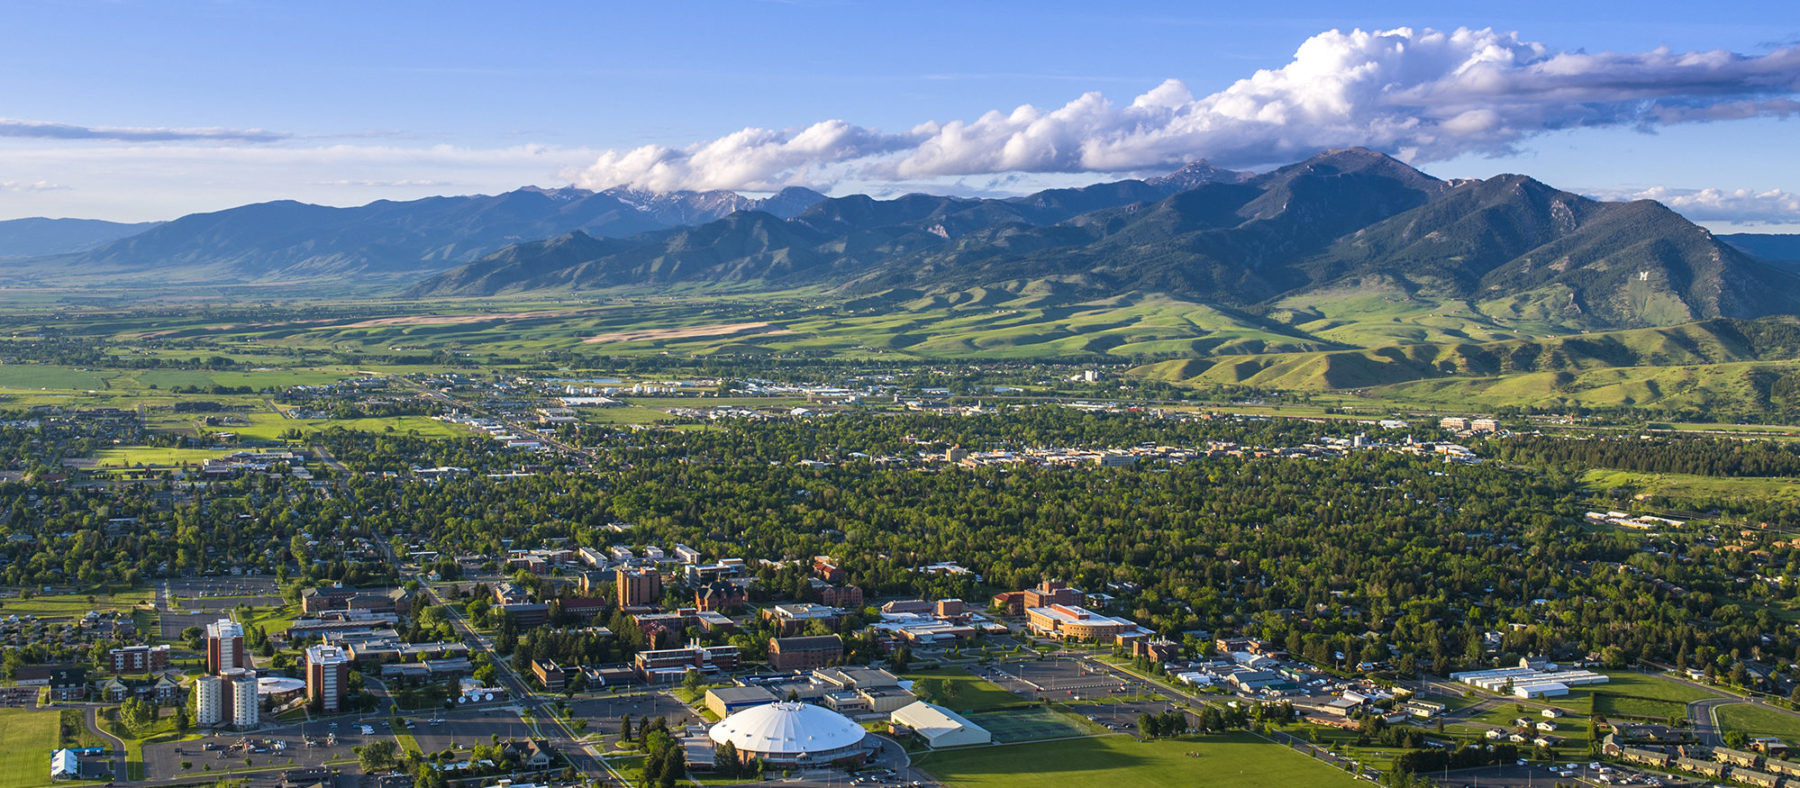
\includegraphics[width=5in,height=\textheight]{images/msu-campus.jpg}}
\usepackage{etoolbox}
\makeatletter
\providecommand{\subtitle}[1]{% add subtitle to \maketitle
  \apptocmd{\@title}{\par {\large #1 \par}}{}{}
}
\makeatother
\subtitle{Spring 2025\\
Montana State University}
\author{Melinda Yager\\
Jade Schmidt\\
Stacey Hancock}
\date{}

\begin{document}
\maketitle

\chapter*{Preface}\label{preface}
\addcontentsline{toc}{chapter}{Preface}

Placeholder

\chapter{Basics of Data and Sampling Methods}\label{basics-of-data-and-sampling-methods}

Placeholder

\section{Vocabulary Review and Key Topics}\label{vocabulary-review-and-key-topics}

\subsection{Key topics}\label{key-topics}

\subsection{Vocabulary}\label{vocabulary}

\section{Activity 1: Intro to Data}\label{activity-1-intro-to-data}

\subsection{Learning outcomes}\label{learning-outcomes}

\subsection{Terminology review}\label{terminology-review}

\subsection{General information on the Coursepack}\label{general-information-on-the-coursepack}

\subsection{Steps of the statistical investigation process}\label{steps-of-the-statistical-investigation-process}

\subsection{Take-home messages}\label{take-home-messages}

\subsection{Additional notes}\label{additional-notes}

\section{Video Notes: Intro to data and Sampling Methods}\label{video-notes-intro-to-data-and-sampling-methods}

\subsection{Course Videos}\label{course-videos}

\subsection*{Data basics: Video 1.2.1and1.2.2}\label{data-basics-video-1.2.1and1.2.2}
\addcontentsline{toc}{subsection}{Data basics: Video 1.2.1and1.2.2}

\subsubsection*{Types of variables}\label{types-of-variables}
\addcontentsline{toc}{subsubsection}{Types of variables}

\subsubsection*{Exploratory data analysis (EDA)}\label{exploratory-data-analysis-eda}
\addcontentsline{toc}{subsubsection}{Exploratory data analysis (EDA)}

\subsection*{Roles of variables: 1.2.3to1.2.4}\label{roles-of-variables-1.2.3to1.2.4}
\addcontentsline{toc}{subsection}{Roles of variables: 1.2.3to1.2.4}

\subsubsection*{Relationships between variables}\label{relationships-between-variables}
\addcontentsline{toc}{subsubsection}{Relationships between variables}

\subsection{Concept Check}\label{concept-check}

\subsection*{Sampling Methods: Video 2.1}\label{sampling-methods-video-2.1}
\addcontentsline{toc}{subsection}{Sampling Methods: Video 2.1}

\subsubsection*{Good vs.~bad sampling}\label{good-vs.-bad-sampling}
\addcontentsline{toc}{subsubsection}{Good vs.~bad sampling}

\subsection*{Types of Sampling Bias}\label{types-of-sampling-bias}
\addcontentsline{toc}{subsection}{Types of Sampling Bias}

\subsubsection*{Video Example}\label{video-example}
\addcontentsline{toc}{subsubsection}{Video Example}

\subsection{Concept Check}\label{concept-check-1}

\section{Activity 2: Intro to Data Analysis and Sampling Bias}\label{activity-2-intro-to-data-analysis-and-sampling-bias}

\subsection{Learning outcomes}\label{learning-outcomes-1}

\subsection{Terminology review}\label{terminology-review-1}

\subsubsection*{Further analysis of class data set}\label{further-analysis-of-class-data-set}
\addcontentsline{toc}{subsubsection}{Further analysis of class data set}

\subsection{Sampling Methods}\label{sampling-methods}

\subsubsection*{Types of bias}\label{types-of-bias}
\addcontentsline{toc}{subsubsection}{Types of bias}

\subsection{Take-home messages}\label{take-home-messages-1}

\subsection{Additional notes}\label{additional-notes-1}

\section{Activity 3: American Indian Address}\label{activity-3-american-indian-address}

\subsection{Learning outcomes}\label{learning-outcomes-2}

\subsection{Terminology review}\label{terminology-review-2}

\subsection{Class Preparation}\label{class-preparation}

\subsection{American Indian Address}\label{american-indian-address}

\subsubsection*{By eye selection}\label{by-eye-selection}
\addcontentsline{toc}{subsubsection}{By eye selection}

\subsection{Class Activity}\label{class-activity}

\subsubsection*{Random selection}\label{random-selection}
\addcontentsline{toc}{subsubsection}{Random selection}

\subsection*{Effect of sample size}\label{effect-of-sample-size}
\addcontentsline{toc}{subsection}{Effect of sample size}

\subsection{Take-home messages}\label{take-home-messages-2}

\subsection{Additional notes}\label{additional-notes-2}

\chapter{Probability}\label{probability}

Placeholder

\section{Vocabulary Review and Key Topics}\label{vocabulary-review-and-key-topics-1}

\subsection{Key topics}\label{key-topics-1}

\subsection{Vocabulary}\label{vocabulary-1}

\section{Video Notes: Probability}\label{video-notes-probability}

\subsection{Course Videos}\label{course-videos-1}

\subsection*{Probability}\label{probability-1}
\addcontentsline{toc}{subsection}{Probability}

\subsubsection*{Creating a hypothetical two-way table}\label{creating-a-hypothetical-two-way-table}
\addcontentsline{toc}{subsubsection}{Creating a hypothetical two-way table}

\subsubsection*{Diagnostic tests}\label{diagnostic-tests}
\addcontentsline{toc}{subsubsection}{Diagnostic tests}

\subsection{Concept Check}\label{concept-check-2}

\section{Activity 4: Probability Studies}\label{activity-4-probability-studies}

\subsection{Learning outcomes}\label{learning-outcomes-3}

\subsection{Terminology review}\label{terminology-review-3}

\subsection{Overview of probabiliy}\label{overview-of-probabiliy}

\subsubsection*{Probability notation}\label{probability-notation}
\addcontentsline{toc}{subsubsection}{Probability notation}

\subsubsection{Probability questions}\label{probability-questions}

\subsection{Calculating probabilities from a two-way table}\label{calculating-probabilities-from-a-two-way-table}

\subsection{Take home messages}\label{take-home-messages-3}

\subsection{Additional notes}\label{additional-notes-3}

\section{Activity 5: What's the probability?}\label{activity-5-whats-the-probability}

\subsection{Learning outcomes}\label{learning-outcomes-4}

\subsection{Terminology review}\label{terminology-review-4}

\subsection{Probability}\label{probability-2}

\subsection{Take home messages}\label{take-home-messages-4}

\subsection{Additional notes}\label{additional-notes-4}

\chapter{Exploring Categorical Data: Exploratory Data Analysis and Inference using Simulation-based Methods}\label{exploring-categorical-data-exploratory-data-analysis-and-inference-using-simulation-based-methods}

Placeholder

\section{Vocabulary Review and Key Topics}\label{vocabulary-review-and-key-topics-2}

\subsection{Key topics}\label{key-topics-2}

\subsubsection*{Steps of the statistical investigation process}\label{steps-of-the-statistical-investigation-process-1}
\addcontentsline{toc}{subsubsection}{Steps of the statistical investigation process}

\subsection{Vocabulary}\label{vocabulary-2}

\subsubsection*{Plotting one categorical variable}\label{plotting-one-categorical-variable}
\addcontentsline{toc}{subsubsection}{Plotting one categorical variable}

\subsubsection*{Inference}\label{inference}
\addcontentsline{toc}{subsubsection}{Inference}

\subsubsection{Simulation-based inference for a single proportion}\label{simulation-based-inference-for-a-single-proportion}

\section{Video Notes: Exploratory Data Analysis of Categorical Variables}\label{video-notes-exploratory-data-analysis-of-categorical-variables}

\subsection{Course Videos}\label{course-videos-2}

\subsection*{Summarizing categorical data - Video 4.1\_OneProp}\label{summarizing-categorical-data---video-4.1_oneprop}
\addcontentsline{toc}{subsection}{Summarizing categorical data - Video 4.1\_OneProp}

\subsubsection*{Displaying categorical variables - Video 4.2\_OneProp}\label{displaying-categorical-variables---video-4.2_oneprop}
\addcontentsline{toc}{subsubsection}{Displaying categorical variables - Video 4.2\_OneProp}

\subsection*{Hypothesis Testing - Video Chapter9}\label{hypothesis-testing---video-chapter9}
\addcontentsline{toc}{subsection}{Hypothesis Testing - Video Chapter9}

\subsection*{Hypothesis Testing/Justice System}\label{hypothesis-testingjustice-system}
\addcontentsline{toc}{subsection}{Hypothesis Testing/Justice System}

\subsubsection*{Null hypothesis}\label{null-hypothesis}
\addcontentsline{toc}{subsubsection}{Null hypothesis}

\subsubsection*{Alternative hypothesis}\label{alternative-hypothesis}
\addcontentsline{toc}{subsubsection}{Alternative hypothesis}

\subsection*{Simulation vs.~Theory-based Methods}\label{simulation-vs.-theory-based-methods}
\addcontentsline{toc}{subsection}{Simulation vs.~Theory-based Methods}

\subsubsection*{Simulation-based method}\label{simulation-based-method}
\addcontentsline{toc}{subsubsection}{Simulation-based method}

\subsubsection*{Theory-based method}\label{theory-based-method}
\addcontentsline{toc}{subsubsection}{Theory-based method}

\subsubsection*{P-value}\label{p-value}
\addcontentsline{toc}{subsubsection}{P-value}

\subsection*{One proportion test}\label{one-proportion-test}
\addcontentsline{toc}{subsection}{One proportion test}

\subsubsection*{Hypothesis testing}\label{hypothesis-testing}
\addcontentsline{toc}{subsubsection}{Hypothesis testing}

\subsubsection*{Simulation-based method}\label{simulation-based-method-1}
\addcontentsline{toc}{subsubsection}{Simulation-based method}

\subsection*{Confidence interval - Video Chapter10}\label{confidence-interval---video-chapter10}
\addcontentsline{toc}{subsection}{Confidence interval - Video Chapter10}

\subsubsection*{Sampling distribution}\label{sampling-distribution}
\addcontentsline{toc}{subsubsection}{Sampling distribution}

\subsubsection*{Simulation-based methods}\label{simulation-based-methods}
\addcontentsline{toc}{subsubsection}{Simulation-based methods}

\subsubsection*{Video 14.2}\label{video-14.2}
\addcontentsline{toc}{subsubsection}{Video 14.2}

\subsection{Concept Check}\label{concept-check-3}

\section{Activity 6: Helper-Hinderer Part 1 --- Simulation-based Hypothesis Test}\label{activity-6-helper-hinderer-part-1-simulation-based-hypothesis-test}

\subsection{Learning outcomes}\label{learning-outcomes-5}

\subsection{Terminology review}\label{terminology-review-5}

\subsection{Steps of the statistical investigation process}\label{steps-of-the-statistical-investigation-process-2}

\subsection{Helper-Hinderer}\label{helper-hinderer}

\subsubsection*{Ask a research question}\label{ask-a-research-question}
\addcontentsline{toc}{subsubsection}{Ask a research question}

\subsubsection*{Design a study and collect data}\label{design-a-study-and-collect-data}
\addcontentsline{toc}{subsubsection}{Design a study and collect data}

\subsubsection*{R code}\label{r-code}
\addcontentsline{toc}{subsubsection}{R code}

\subsubsection*{Summarize and visualize the data}\label{summarize-and-visualize-the-data}
\addcontentsline{toc}{subsubsection}{Summarize and visualize the data}

\subsubsection*{Use statistical analysis methods to draw inferences from the data}\label{use-statistical-analysis-methods-to-draw-inferences-from-the-data}
\addcontentsline{toc}{subsubsection}{Use statistical analysis methods to draw inferences from the data}

\subsection{Take-home messages}\label{take-home-messages-5}

\subsection{Additional notes}\label{additional-notes-5}

\section{Activity 7: Helper-Hinderer (continued)}\label{activity-7-helper-hinderer-continued}

\subsection{Learning outcomes}\label{learning-outcomes-6}

\subsection{Steps of the statistical investigation process}\label{steps-of-the-statistical-investigation-process-3}

\subsection{Helper-Hinderer}\label{helper-hinderer-1}

\subsubsection*{Interpret the p-value}\label{interpret-the-p-value}
\addcontentsline{toc}{subsubsection}{Interpret the p-value}

\subsubsection*{Communicate the results and answer the research question}\label{communicate-the-results-and-answer-the-research-question}
\addcontentsline{toc}{subsubsection}{Communicate the results and answer the research question}

\subsection{Take-home messages}\label{take-home-messages-6}

\subsection{Additional notes}\label{additional-notes-6}

\section{Activity 8: Helper-Hinderer --- Simulation-based Confidence Interval}\label{activity-8-helper-hinderer-simulation-based-confidence-interval}

\subsection{Learning outcomes}\label{learning-outcomes-7}

\subsection{Terminology review}\label{terminology-review-6}

\subsection{Helper-Hinderer}\label{helper-hinderer-2}

\subsubsection*{Activity intro}\label{activity-intro}
\addcontentsline{toc}{subsubsection}{Activity intro}

\subsubsection*{Use statistical analysis methods to draw inferences from the data}\label{use-statistical-analysis-methods-to-draw-inferences-from-the-data-1}
\addcontentsline{toc}{subsubsection}{Use statistical analysis methods to draw inferences from the data}

\subsubsection*{Communicate the results and answer the research question}\label{communicate-the-results-and-answer-the-research-question-1}
\addcontentsline{toc}{subsubsection}{Communicate the results and answer the research question}

\subsubsection*{Effect of confidence level}\label{effect-of-confidence-level}
\addcontentsline{toc}{subsubsection}{Effect of confidence level}

\subsection{Take-home messages}\label{take-home-messages-7}

\subsection{Additional notes}\label{additional-notes-7}

\chapter{Inference for a Single Categorical Variable: Theory-based Methods}\label{inference-for-a-single-categorical-variable-theory-based-methods}

Placeholder

\section{Vocabulary Review and Key Topics}\label{vocabulary-review-and-key-topics-3}

\subsection{Key topics}\label{key-topics-3}

\subsection{Vocabulary}\label{vocabulary-3}

\section{Video Notes: Inference for One Categorical Variable using Theory-based Methods}\label{video-notes-inference-for-one-categorical-variable-using-theory-based-methods}

\subsection{Course Videos}\label{course-videos-3}

\subsection*{Theory-based methods}\label{theory-based-methods}
\addcontentsline{toc}{subsection}{Theory-based methods}

\subsubsection*{Central limit theorem - Video Chapter11}\label{central-limit-theorem---video-chapter11}
\addcontentsline{toc}{subsubsection}{Central limit theorem - Video Chapter11}

\subsection*{68-95-99.7 Rule}\label{rule}
\addcontentsline{toc}{subsection}{68-95-99.7 Rule}

\subsubsection*{Example in Video 14.3TheoryTests}\label{example-in-video-14.3theorytests}
\addcontentsline{toc}{subsubsection}{Example in Video 14.3TheoryTests}

\subsection*{Confidence interval - 14.3TheoryIntervals}\label{confidence-interval---14.3theoryintervals}
\addcontentsline{toc}{subsection}{Confidence interval - 14.3TheoryIntervals}

\subsubsection*{Theory-based method for a single categorical variable}\label{theory-based-method-for-a-single-categorical-variable}
\addcontentsline{toc}{subsubsection}{Theory-based method for a single categorical variable}

\subsubsection*{Interpreting confidence level}\label{interpreting-confidence-level}
\addcontentsline{toc}{subsubsection}{Interpreting confidence level}

\subsection{Concept Check}\label{concept-check-4}

\section{Activity 9: Handedness of Male Boxers}\label{activity-9-handedness-of-male-boxers}

\subsection{Learning outcomes}\label{learning-outcomes-8}

\subsection{Terminology review}\label{terminology-review-7}

\subsection{Handedness of male boxers}\label{handedness-of-male-boxers}

\subsection{Summary statistics review}\label{summary-statistics-review}

\subsection*{Hypotheses and summary statistics}\label{hypotheses-and-summary-statistics}
\addcontentsline{toc}{subsection}{Hypotheses and summary statistics}

\subsection*{Theory-based methods}\label{theory-based-methods-1}
\addcontentsline{toc}{subsection}{Theory-based methods}

\subsection*{Impacts on the P-value}\label{impacts-on-the-p-value}
\addcontentsline{toc}{subsection}{Impacts on the P-value}

\subsection{Take-home messages}\label{take-home-messages-8}

\subsection{Additional notes}\label{additional-notes-8}

\section{Activity 10: Confidence interval and what confidence means}\label{activity-10-confidence-interval-and-what-confidence-means}

\subsection{Learning outcomes}\label{learning-outcomes-9}

\subsection{Terminology review}\label{terminology-review-8}

\subsection{Handedness of male boxers continued}\label{handedness-of-male-boxers-continued}

\subsection*{\texorpdfstring{What does \emph{confidence} mean?}{What does confidence mean?}}\label{what-does-confidence-mean}
\addcontentsline{toc}{subsection}{What does \emph{confidence} mean?}

\subsubsection*{Theory-based confidence interval}\label{theory-based-confidence-interval}
\addcontentsline{toc}{subsubsection}{Theory-based confidence interval}

\subsection{Take-home messages}\label{take-home-messages-9}

\subsection{Additional notes}\label{additional-notes-9}

\section{Module 3 and 4 Lab: Mixed Breed Dogs in the U.S.}\label{module-3-and-4-lab-mixed-breed-dogs-in-the-u.s.}

\subsection{Learning outcomes}\label{learning-outcomes-10}

\subsection{Mixed Breed Dogs in the U.S.}\label{mixed-breed-dogs-in-the-u.s.}

\subsubsection*{Activity intro}\label{activity-intro-1}
\addcontentsline{toc}{subsubsection}{Activity intro}

\subsubsection*{Use statistical analysis methods to draw inferences from the data}\label{use-statistical-analysis-methods-to-draw-inferences-from-the-data-2}
\addcontentsline{toc}{subsubsection}{Use statistical analysis methods to draw inferences from the data}

\subsubsection*{Summarize the results of the study}\label{summarize-the-results-of-the-study}
\addcontentsline{toc}{subsubsection}{Summarize the results of the study}

\chapter{Unit 1 Review}\label{unit-1-review}

The following module contains both a list of key topics covered in Unit 1 as well as Module Review Worksheets that will be covered in Weekly Review Sessions.

\subsection{Key Topics}\label{key-topics-4}

Review the key topics for Unit 1 prior to the first exams. All of these topics will be covered in Modules 1--4.

\subsection{Module Review}\label{module-review}

\setstretch{1}

The following worksheets review each of the modules. These worksheets will be completed during Melinda's Study Sessions each week. Solutions will be posted on D2L in the Unit 1 Review folder after the study sessions.

\newpage

\section{Key Topics Exam 1}\label{key-topics-exam-1}

\subsection*{Descriptive statistics and study design}\label{descriptive-statistics-and-study-design}
\addcontentsline{toc}{subsection}{Descriptive statistics and study design}

\subsection*{Hypothesis testing}\label{hypothesis-testing-1}
\addcontentsline{toc}{subsection}{Hypothesis testing}

\subsection{Confidence intervals}\label{confidence-intervals}

\subsection{Probability}\label{probability-3}

\section{Module 1 Review - Sampling Methods}\label{module-1-review---sampling-methods}

\section{Module 2 Review - Probability}\label{module-2-review---probability}

\section{Module 3 Review - Simulation Methods for a Single Proportion}\label{module-3-review---simulation-methods-for-a-single-proportion}

\section{Module 4 Review - Theory-based Methods for a Single Proportion}\label{module-4-review---theory-based-methods-for-a-single-proportion}

\chapter{Exploring Quantitative Data: Exploratory Data Analysis and Hypothesis Testing for a Single Quantitative Variable}\label{exploring-quantitative-data-exploratory-data-analysis-and-hypothesis-testing-for-a-single-quantitative-variable}

Placeholder

\section{Vocabulary Review and Key Topics}\label{vocabulary-review-and-key-topics-4}

\subsection{Key topics}\label{key-topics-5}

\subsection{Vocabulary}\label{vocabulary-4}

\subsubsection*{Sample statistics for a single quantitative variable}\label{sample-statistics-for-a-single-quantitative-variable}
\addcontentsline{toc}{subsubsection}{Sample statistics for a single quantitative variable}

\subsubsection*{Plotting one quantitative variable}\label{plotting-one-quantitative-variable}
\addcontentsline{toc}{subsubsection}{Plotting one quantitative variable}

\subsubsection*{Hypothesis testing for a single mean}\label{hypothesis-testing-for-a-single-mean}
\addcontentsline{toc}{subsubsection}{Hypothesis testing for a single mean}

\subsubsection*{Simulation-based hypothesis testing}\label{simulation-based-hypothesis-testing}
\addcontentsline{toc}{subsubsection}{Simulation-based hypothesis testing}

\subsubsection*{Theory-based hypothesis testing}\label{theory-based-hypothesis-testing}
\addcontentsline{toc}{subsubsection}{Theory-based hypothesis testing}

\section{Video Notes: Exploratory Data Analysis and Hypothesis Testing of Quantitative Variables}\label{video-notes-exploratory-data-analysis-and-hypothesis-testing-of-quantitative-variables}

\subsection{Course Videos}\label{course-videos-4}

\subsection*{Summarizing quantitative data - Videos 5.2to5.4 and 5.5to5.6}\label{summarizing-quantitative-data---videos-5.2to5.4-and-5.5to5.6}
\addcontentsline{toc}{subsection}{Summarizing quantitative data - Videos 5.2to5.4 and 5.5to5.6}

\subsubsection*{Types of plots}\label{types-of-plots}
\addcontentsline{toc}{subsubsection}{Types of plots}

\subsubsection*{Four characteristics of plots for quantitative variables}\label{four-characteristics-of-plots-for-quantitative-variables}
\addcontentsline{toc}{subsubsection}{Four characteristics of plots for quantitative variables}

\subsubsection*{Robust statistics - Video 5.7}\label{robust-statistics---video-5.7}
\addcontentsline{toc}{subsubsection}{Robust statistics - Video 5.7}

\subsection{Video notes single quantitative variable inference}\label{video-notes-single-quantitative-variable-inference}

\subsection*{Hypothesis testing}\label{hypothesis-testing-2}
\addcontentsline{toc}{subsection}{Hypothesis testing}

\subsubsection*{Simulation-based method}\label{simulation-based-method-2}
\addcontentsline{toc}{subsubsection}{Simulation-based method}

\subsubsection*{Theory-based method}\label{theory-based-method-1}
\addcontentsline{toc}{subsubsection}{Theory-based method}

\subsection*{\texorpdfstring{\(t\)-distribution}{t-distribution}}\label{t-distribution}
\addcontentsline{toc}{subsection}{\(t\)-distribution}

\subsection{Concept Check}\label{concept-check-5}

\section{Activity 11: Summarizing Quantitative Variables}\label{activity-11-summarizing-quantitative-variables}

\subsection{Learning outcomes}\label{learning-outcomes-11}

\subsection{Terminology review}\label{terminology-review-9}

\subsection{The Integrated Postsecondary Education Data System (IPEDS)}\label{the-integrated-postsecondary-education-data-system-ipeds}

\subsubsection*{Identifying variables in a data set}\label{identifying-variables-in-a-data-set}
\addcontentsline{toc}{subsubsection}{Identifying variables in a data set}

\subsubsection*{Summarizing quantitative variables}\label{summarizing-quantitative-variables}
\addcontentsline{toc}{subsubsection}{Summarizing quantitative variables}

\subsubsection*{Displaying a single quantitative variable}\label{displaying-a-single-quantitative-variable}
\addcontentsline{toc}{subsubsection}{Displaying a single quantitative variable}

\subsubsection*{Robust statistics}\label{robust-statistics}
\addcontentsline{toc}{subsubsection}{Robust statistics}

\subsection{Take-home messages}\label{take-home-messages-10}

\subsection{Additional notes}\label{additional-notes-10}

\section{Activity 12: Hypothesis Testing of a Single Quantitative Variable}\label{activity-12-hypothesis-testing-of-a-single-quantitative-variable}

\subsection{Learning outcomes}\label{learning-outcomes-12}

\subsection{Terminology review}\label{terminology-review-10}

\subsection{College student sleep habits}\label{college-student-sleep-habits}

\subsubsection*{Summarizing quantitative variables}\label{summarizing-quantitative-variables-1}
\addcontentsline{toc}{subsubsection}{Summarizing quantitative variables}

\subsubsection*{Ask a research question}\label{ask-a-research-question-1}
\addcontentsline{toc}{subsubsection}{Ask a research question}

\subsubsection*{Summarize and visualize the data}\label{summarize-and-visualize-the-data-1}
\addcontentsline{toc}{subsubsection}{Summarize and visualize the data}

\subsection*{Simulation methods}\label{simulation-methods}
\addcontentsline{toc}{subsection}{Simulation methods}

\subsection{Take-home messages}\label{take-home-messages-11}

\subsection{Additional notes}\label{additional-notes-11}

\section{Activity 13: Body Temperature}\label{activity-13-body-temperature}

\subsection{Learning outcomes}\label{learning-outcomes-13}

\subsection{Terminology review}\label{terminology-review-11}

\subsection{Body Temperature}\label{body-temperature}

\subsubsection*{Ask a research question}\label{ask-a-research-question-2}
\addcontentsline{toc}{subsubsection}{Ask a research question}

\subsubsection*{Summarize and visualize the data}\label{summarize-and-visualize-the-data-2}
\addcontentsline{toc}{subsubsection}{Summarize and visualize the data}

\subsubsection*{Check theoretical conditions}\label{check-theoretical-conditions}
\addcontentsline{toc}{subsubsection}{Check theoretical conditions}

\subsubsection*{Use statistical inferential methods to draw inferences from the data}\label{use-statistical-inferential-methods-to-draw-inferences-from-the-data}
\addcontentsline{toc}{subsubsection}{Use statistical inferential methods to draw inferences from the data}

\subsection{Take-home messages}\label{take-home-messages-12}

\subsection{Additional notes}\label{additional-notes-12}

\chapter{Confidence Intervals for a Single Quantitative Variable}\label{confidence-intervals-for-a-single-quantitative-variable}

Placeholder

\section{Vocabulary Review and Key Topics}\label{vocabulary-review-and-key-topics-5}

\subsection{Key topics}\label{key-topics-6}

\subsubsection*{Simulation-based confidence interval}\label{simulation-based-confidence-interval}
\addcontentsline{toc}{subsubsection}{Simulation-based confidence interval}

\subsubsection*{Theory-based confidence interval}\label{theory-based-confidence-interval-1}
\addcontentsline{toc}{subsubsection}{Theory-based confidence interval}

\subsection*{Vocabulary}\label{vocabulary-5}
\addcontentsline{toc}{subsection}{Vocabulary}

\section{Video Notes: Theory-based Inference for a single quantitative variable}\label{video-notes-theory-based-inference-for-a-single-quantitative-variable}

\subsection{Course Videos}\label{course-videos-5}

\subsection{Single quantitative variable}\label{single-quantitative-variable}

\subsection*{Confidence interval}\label{confidence-interval}
\addcontentsline{toc}{subsection}{Confidence interval}

\subsubsection*{Simulation-based method}\label{simulation-based-method-3}
\addcontentsline{toc}{subsubsection}{Simulation-based method}

\subsubsection*{Theory-based method}\label{theory-based-method-2}
\addcontentsline{toc}{subsubsection}{Theory-based method}

\subsection*{\texorpdfstring{\(t\)-distribution}{t-distribution}}\label{t-distribution-1}
\addcontentsline{toc}{subsection}{\(t\)-distribution}

\subsection{Concept Check}\label{concept-check-6}

\section{Activity 14: Danceability of Songs}\label{activity-14-danceability-of-songs}

\subsection{Learning outcomes}\label{learning-outcomes-14}

\subsection{Terminology review}\label{terminology-review-12}

\subsection{Danceability}\label{danceability}

\subsubsection*{Summarizing quantitative variables}\label{summarizing-quantitative-variables-2}
\addcontentsline{toc}{subsubsection}{Summarizing quantitative variables}

\subsection*{Simulation methods to create a confidence interval}\label{simulation-methods-to-create-a-confidence-interval}
\addcontentsline{toc}{subsection}{Simulation methods to create a confidence interval}

\subsection*{Theory-based methods to create a confidence interval}\label{theory-based-methods-to-create-a-confidence-interval}
\addcontentsline{toc}{subsection}{Theory-based methods to create a confidence interval}

\subsection{Take-home messages}\label{take-home-messages-13}

\subsection{Additional notes}\label{additional-notes-13}

\section{Activity 15: Errors and Power}\label{activity-15-errors-and-power}

\subsection{Learning outcomes}\label{learning-outcomes-15}

\subsection{Terminology review}\label{terminology-review-13}

\subsection{College textbook cost}\label{college-textbook-cost}

\subsection{Take-home messages}\label{take-home-messages-14}

\subsection{Additional notes}\label{additional-notes-14}

\section{Module 6 and 7 Lab: Arsenic}\label{module-6-and-7-lab-arsenic}

\subsection{Learning outcomes}\label{learning-outcomes-16}

\subsection{Arsenic}\label{arsenic}

\subsection*{Use statistical inferential methods to draw inferences from the data}\label{use-statistical-inferential-methods-to-draw-inferences-from-the-data-1}
\addcontentsline{toc}{subsection}{Use statistical inferential methods to draw inferences from the data}

\subsection*{Hypothesis test}\label{hypothesis-test}
\addcontentsline{toc}{subsection}{Hypothesis test}

\subsection*{Communicate the results and answer the research question}\label{communicate-the-results-and-answer-the-research-question-2}
\addcontentsline{toc}{subsection}{Communicate the results and answer the research question}

\subsection*{Confidence interval}\label{confidence-interval-1}
\addcontentsline{toc}{subsection}{Confidence interval}

\chapter{Exploratory Data Analysis and Simulation-based Hypothesis Testing for Two Categorical Variables}\label{exploratory-data-analysis-and-simulation-based-hypothesis-testing-for-two-categorical-variables}

Placeholder

\section{Vocabulary Review and Key Topics}\label{vocabulary-review-and-key-topics-6}

\subsection{Key topics}\label{key-topics-7}

\subsection{Vocabulary}\label{vocabulary-6}

\subsubsection*{Sample statistics for two categorical variables}\label{sample-statistics-for-two-categorical-variables}
\addcontentsline{toc}{subsubsection}{Sample statistics for two categorical variables}

\subsubsection*{Plotting two categorical variables}\label{plotting-two-categorical-variables}
\addcontentsline{toc}{subsubsection}{Plotting two categorical variables}

\subsubsection*{Hypotheses}\label{hypotheses}
\addcontentsline{toc}{subsubsection}{Hypotheses}

\subsubsection*{Simulation-based hypothesis testing for a difference in proportions}\label{simulation-based-hypothesis-testing-for-a-difference-in-proportions}
\addcontentsline{toc}{subsubsection}{Simulation-based hypothesis testing for a difference in proportions}

\subsubsection*{Study design}\label{study-design}
\addcontentsline{toc}{subsubsection}{Study design}

\subsubsection{Scope of inference}\label{scope-of-inference}

\section{Video Notes: Inference for Two Categorical Variables using Simulation-based Methods}\label{video-notes-inference-for-two-categorical-variables-using-simulation-based-methods}

\subsection{Course Videos}\label{course-videos-6}

\subsection*{Observational studies, experiments, and scope of inference: Video 2.2to2.4}\label{observational-studies-experiments-and-scope-of-inference-video-2.2to2.4}
\addcontentsline{toc}{subsection}{Observational studies, experiments, and scope of inference: Video 2.2to2.4}

\subsubsection*{Study design}\label{study-design-1}
\addcontentsline{toc}{subsubsection}{Study design}

\subsubsection*{Scope of Inference}\label{scope-of-inference-1}
\addcontentsline{toc}{subsubsection}{Scope of Inference}

\subsection*{Summarizing two categorical variables - Video 4.1\_TwoProp}\label{summarizing-two-categorical-variables---video-4.1_twoprop}
\addcontentsline{toc}{subsection}{Summarizing two categorical variables - Video 4.1\_TwoProp}

\subsection*{Plots for two categorical variables - Video 4.2\_TwoProp}\label{plots-for-two-categorical-variables---video-4.2_twoprop}
\addcontentsline{toc}{subsection}{Plots for two categorical variables - Video 4.2\_TwoProp}

\subsubsection*{Simpson's paradox - Video 4.4}\label{simpsons-paradox---video-4.4}
\addcontentsline{toc}{subsubsection}{Simpson's paradox - Video 4.4}

\subsection*{Two categorical variables - Video 15.1}\label{two-categorical-variables---video-15.1}
\addcontentsline{toc}{subsection}{Two categorical variables - Video 15.1}

\subsection*{Hypothesis Testing}\label{hypothesis-testing-3}
\addcontentsline{toc}{subsection}{Hypothesis Testing}

\subsubsection*{Summary statistics and plot}\label{summary-statistics-and-plot}
\addcontentsline{toc}{subsubsection}{Summary statistics and plot}

\subsubsection*{Simulation-based method}\label{simulation-based-method-4}
\addcontentsline{toc}{subsubsection}{Simulation-based method}

\subsection*{Confidence interval - Video 15.2}\label{confidence-interval---video-15.2}
\addcontentsline{toc}{subsection}{Confidence interval - Video 15.2}

\subsubsection*{Simulation-based method}\label{simulation-based-method-5}
\addcontentsline{toc}{subsubsection}{Simulation-based method}

\subsection*{Relative Risk - Video RelativeRisk}\label{relative-risk---video-relativerisk}
\addcontentsline{toc}{subsection}{Relative Risk - Video RelativeRisk}

\subsubsection*{Relative risk in the news}\label{relative-risk-in-the-news}
\addcontentsline{toc}{subsubsection}{Relative risk in the news}

\subsubsection*{Testing Relative Risk}\label{testing-relative-risk}
\addcontentsline{toc}{subsubsection}{Testing Relative Risk}

\subsection{Concept Check}\label{concept-check-7}

\section{Activity 16: Study Design}\label{activity-16-study-design}

\subsection{Learning outcomes}\label{learning-outcomes-17}

\subsection{Terminology review}\label{terminology-review-14}

\subsection{Atrial fibrillation}\label{atrial-fibrillation}

\subsection{Scope of Inference}\label{scope-of-inference-2}

\subsection{Take-home messages}\label{take-home-messages-15}

\subsection{Additional notes}\label{additional-notes-15}

\section{Activity 17: Summarizing Two Categorical Variables}\label{activity-17-summarizing-two-categorical-variables}

\subsection{Learning outcomes}\label{learning-outcomes-18}

\subsection{Terminology review}\label{terminology-review-15}

\subsection{Graphing categorical variables}\label{graphing-categorical-variables}

\subsection*{Nightlight use and myopia}\label{nightlight-use-and-myopia}
\addcontentsline{toc}{subsection}{Nightlight use and myopia}

\subsubsection*{R code}\label{r-code-1}
\addcontentsline{toc}{subsubsection}{R code}

\subsubsection*{Summarizing two categorical variables}\label{summarizing-two-categorical-variables}
\addcontentsline{toc}{subsubsection}{Summarizing two categorical variables}

\subsubsection*{Displaying two categorical variables}\label{displaying-two-categorical-variables}
\addcontentsline{toc}{subsubsection}{Displaying two categorical variables}

\subsubsection*{Relative Risk}\label{relative-risk}
\addcontentsline{toc}{subsubsection}{Relative Risk}

\subsection{Take-home messages}\label{take-home-messages-16}

\subsection{Additional notes}\label{additional-notes-16}

\section{Activity 18: The Good Samaritan}\label{activity-18-the-good-samaritan}

\subsection{Learning outcomes}\label{learning-outcomes-19}

\subsection{Terminology review}\label{terminology-review-16}

\subsection{The Good Samaritan}\label{the-good-samaritan}

\subsubsection*{Ask a research question}\label{ask-a-research-question-3}
\addcontentsline{toc}{subsubsection}{Ask a research question}

\subsubsection*{Summarize and visualize the data}\label{summarize-and-visualize-the-data-3}
\addcontentsline{toc}{subsubsection}{Summarize and visualize the data}

\subsubsection*{Hypothesis Test}\label{hypothesis-test-1}
\addcontentsline{toc}{subsubsection}{Hypothesis Test}

\subsection{Take-home messages}\label{take-home-messages-17}

\subsection{Additional notes}\label{additional-notes-17}

\chapter{Theory-based Hypothesis Testing and Simulation-based and Theory-based Confidence Intervals for Two Categorical Variables:}\label{theory-based-hypothesis-testing-and-simulation-based-and-theory-based-confidence-intervals-for-two-categorical-variables}

Placeholder

\section{Vocabulary Review and Key Topics}\label{vocabulary-review-and-key-topics-7}

\subsection{Key topics}\label{key-topics-8}

\subsection{Vocabulary}\label{vocabulary-7}

\subsubsection*{Theory-based inference}\label{theory-based-inference}
\addcontentsline{toc}{subsubsection}{Theory-based inference}

\subsubsection*{Simulation-based confidence interval}\label{simulation-based-confidence-interval-1}
\addcontentsline{toc}{subsubsection}{Simulation-based confidence interval}

\section{Video Notes: Theoretical Inference for Two Categorical Variables}\label{video-notes-theoretical-inference-for-two-categorical-variables}

\subsection{Course Videos}\label{course-videos-7}

\subsection*{Hypothesis testing using theory-based methods - Video 15.4TheoryTests}\label{hypothesis-testing-using-theory-based-methods---video-15.4theorytests}
\addcontentsline{toc}{subsection}{Hypothesis testing using theory-based methods - Video 15.4TheoryTests}

\subsection*{Confidence interval - Video 15.3TheoryIntervals}\label{confidence-interval---video-15.3theoryintervals}
\addcontentsline{toc}{subsection}{Confidence interval - Video 15.3TheoryIntervals}

\subsubsection*{Theory-based method for a two categorical variables}\label{theory-based-method-for-a-two-categorical-variables}
\addcontentsline{toc}{subsubsection}{Theory-based method for a two categorical variables}

\subsection{Concept Check}\label{concept-check-8}

\section{Activity 19: Winter Sports Helmet Use and Head Injuries --- Theory-based Methods}\label{activity-19-winter-sports-helmet-use-and-head-injuries-theory-based-methods}

\subsection{Learning outcomes}\label{learning-outcomes-20}

\subsection{Terminology review}\label{terminology-review-17}

\subsection{Winter sports helmet use and head injury}\label{winter-sports-helmet-use-and-head-injury}

\subsubsection*{Hypothesis test}\label{hypothesis-test-2}
\addcontentsline{toc}{subsubsection}{Hypothesis test}

\subsubsection*{Use statistical analysis methods to draw inferences from the data}\label{use-statistical-analysis-methods-to-draw-inferences-from-the-data-3}
\addcontentsline{toc}{subsubsection}{Use statistical analysis methods to draw inferences from the data}

\subsection*{How would an increase in sample size impact the p-value of the test?}\label{how-would-an-increase-in-sample-size-impact-the-p-value-of-the-test}
\addcontentsline{toc}{subsection}{How would an increase in sample size impact the p-value of the test?}

\subsection{Take-home messages}\label{take-home-messages-18}

\subsection{Additional notes}\label{additional-notes-18}

\section{Activity 20: Diabetes}\label{activity-20-diabetes}

\subsection{Learning outcomes}\label{learning-outcomes-21}

\subsection{Glycemic control in diabetic adolescents}\label{glycemic-control-in-diabetic-adolescents}

\subsection*{Simulation methods}\label{simulation-methods-1}
\addcontentsline{toc}{subsection}{Simulation methods}

\subsection*{Theory-based Methods}\label{theory-based-methods-2}
\addcontentsline{toc}{subsection}{Theory-based Methods}

\subsection{Take-home messages}\label{take-home-messages-19}

\subsection{Additional notes}\label{additional-notes-19}

\section{Module 8 and 9 Lab: Poisonous Mushrooms}\label{module-8-and-9-lab-poisonous-mushrooms}

\subsection{Learning outcomes}\label{learning-outcomes-22}

\subsection{Poisonous Mushrooms}\label{poisonous-mushrooms}

\chapter{Unit 2 Review}\label{unit-2-review}

The following section contains both a list of key topics covered in Unit 2 as well as Module Review Worksheets.

\subsection{Key Topics}\label{key-topics-9}

Review the key topics for Unit 2 to review prior to the exams. All of these topics will be covered in Modules 6--9.

\subsection{Module Review}\label{module-review-1}

\setstretch{1}

The following worksheets review each of the modules. These worksheets will be completed during Melinda's Study Sessions each week. Solutions will be posted on D2L in the Unit 2 Review folder after the study sessions.

\newpage

\section{Key Topics Exam 2}\label{key-topics-exam-2}

\subsection*{Descriptive statistics and study design}\label{descriptive-statistics-and-study-design-1}
\addcontentsline{toc}{subsection}{Descriptive statistics and study design}

\subsection*{Hypothesis testing}\label{hypothesis-testing-4}
\addcontentsline{toc}{subsection}{Hypothesis testing}

\subsection*{Confidence interval}\label{confidence-interval-2}
\addcontentsline{toc}{subsection}{Confidence interval}

\section{Module 6 Review - One Mean Testing}\label{module-6-review---one-mean-testing}

\section{Module 7 Review - One Mean Confidence Interval}\label{module-7-review---one-mean-confidence-interval}

\section{Module 8 - 9 Review - Inference for Two Categorical Variables}\label{module-8---9-review---inference-for-two-categorical-variables}

\chapter{Exploratory Data Analysis and Inference for a Quantitative Response with Paired Samples}\label{exploratory-data-analysis-and-inference-for-a-quantitative-response-with-paired-samples}

Placeholder

\section{Vocabulary Review and Key Topics}\label{vocabulary-review-and-key-topics-8}

\subsection{Key topics}\label{key-topics-10}

\subsection{Vocabulary}\label{vocabulary-8}

\subsubsection*{Simulation-based inference for a paired mean difference}\label{simulation-based-inference-for-a-paired-mean-difference}
\addcontentsline{toc}{subsubsection}{Simulation-based inference for a paired mean difference}

\subsubsection*{Theory-based inference for a paired mean difference}\label{theory-based-inference-for-a-paired-mean-difference}
\addcontentsline{toc}{subsubsection}{Theory-based inference for a paired mean difference}

\section{Video Notes: Inference for Paired Data}\label{video-notes-inference-for-paired-data}

\subsection{Course Videos}\label{course-videos-8}

\subsection*{Single categorical, single quantitative variables Video Paired\_Data}\label{single-categorical-single-quantitative-variables-video-paired_data}
\addcontentsline{toc}{subsection}{Single categorical, single quantitative variables Video Paired\_Data}

\subsection*{Paired vs.~Independent Samples}\label{paired-vs.-independent-samples}
\addcontentsline{toc}{subsection}{Paired vs.~Independent Samples}

\subsection*{Hypothesis testing}\label{hypothesis-testing-5}
\addcontentsline{toc}{subsection}{Hypothesis testing}

\subsubsection*{Simulation-based method}\label{simulation-based-method-6}
\addcontentsline{toc}{subsubsection}{Simulation-based method}

\subsection*{Confidence interval}\label{confidence-interval-3}
\addcontentsline{toc}{subsection}{Confidence interval}

\subsubsection*{Simulation-based method}\label{simulation-based-method-7}
\addcontentsline{toc}{subsubsection}{Simulation-based method}

\subsubsection*{Theory-based method - Video 18.3}\label{theory-based-method---video-18.3}
\addcontentsline{toc}{subsubsection}{Theory-based method - Video 18.3}

\subsubsection*{t-distribution}\label{t-distribution-2}
\addcontentsline{toc}{subsubsection}{t-distribution}

\subsection{Concept Check}\label{concept-check-9}

\section{Activity 21: Paired vs.~Independent Samples}\label{activity-21-paired-vs.-independent-samples}

\subsection{Learning outcomes}\label{learning-outcomes-23}

\subsection{Terminology review}\label{terminology-review-18}

\subsection{Paired vs.~Independent Samples}\label{paired-vs.-independent-samples-1}

\subsection{Tattoo Effect on Sweat Rate}\label{tattoo-effect-on-sweat-rate}

\subsection{Exploring Paired Data}\label{exploring-paired-data}

\subsection{Additional notes}\label{additional-notes-20}

\section{Activity 22: Snakes}\label{activity-22-snakes}

\subsection{Learning outcomes}\label{learning-outcomes-24}

\subsection{Terminology review}\label{terminology-review-19}

\subsection{Snake mazes}\label{snake-mazes}

\subsubsection*{Ask a research question}\label{ask-a-research-question-4}
\addcontentsline{toc}{subsubsection}{Ask a research question}

\subsubsection*{Use statistical inferential methods to draw inferences from the data}\label{use-statistical-inferential-methods-to-draw-inferences-from-the-data-2}
\addcontentsline{toc}{subsubsection}{Use statistical inferential methods to draw inferences from the data}

\paragraph*{Hypothesis test}\label{hypothesis-test-3}
\addcontentsline{toc}{paragraph}{Hypothesis test}

\paragraph*{Confidence interval}\label{confidence-interval-4}
\addcontentsline{toc}{paragraph}{Confidence interval}

\subsection{Take-home messages}\label{take-home-messages-20}

\subsection{Additional notes}\label{additional-notes-21}

\section{Activity 23: Color Interference}\label{activity-23-color-interference}

\subsection{Learning outcomes}\label{learning-outcomes-25}

\subsection{Terminology review}\label{terminology-review-20}

\subsection{Color Interference}\label{color-interference}

\subsubsection*{Identify the scenario}\label{identify-the-scenario}
\addcontentsline{toc}{subsubsection}{Identify the scenario}

\subsubsection*{Ask a research question}\label{ask-a-research-question-5}
\addcontentsline{toc}{subsubsection}{Ask a research question}

\subsubsection*{Summarize and visualize the data}\label{summarize-and-visualize-the-data-4}
\addcontentsline{toc}{subsubsection}{Summarize and visualize the data}

\subsubsection*{Check theoretical conditions}\label{check-theoretical-conditions-1}
\addcontentsline{toc}{subsubsection}{Check theoretical conditions}

\subsubsection*{Use statistical inferential methods to draw inferences from the data}\label{use-statistical-inferential-methods-to-draw-inferences-from-the-data-3}
\addcontentsline{toc}{subsubsection}{Use statistical inferential methods to draw inferences from the data}

\subsection{Take-home messages}\label{take-home-messages-21}

\subsection{Additional notes}\label{additional-notes-22}

\section{Module 11 Lab: Swearing}\label{module-11-lab-swearing}

\subsection{Learning outcomes}\label{learning-outcomes-26}

\subsection{Swearing}\label{swearing}

\subsection*{Use statistical inferential methods to draw inferences from the data}\label{use-statistical-inferential-methods-to-draw-inferences-from-the-data-4}
\addcontentsline{toc}{subsection}{Use statistical inferential methods to draw inferences from the data}

\subsection*{Hypothesis test}\label{hypothesis-test-4}
\addcontentsline{toc}{subsection}{Hypothesis test}

\subsection*{Communicate the results and answer the research question}\label{communicate-the-results-and-answer-the-research-question-3}
\addcontentsline{toc}{subsection}{Communicate the results and answer the research question}

\subsection*{Confidence interval}\label{confidence-interval-5}
\addcontentsline{toc}{subsection}{Confidence interval}

\chapter{Exploratory Data Analysis and Inference for a Quantitative Response with Independent Samples}\label{exploratory-data-analysis-and-inference-for-a-quantitative-response-with-independent-samples}

Placeholder

\section{Vocabulary Review and Key Topics}\label{vocabulary-review-and-key-topics-9}

\subsection{Key topics}\label{key-topics-11}

\subsection{Vocabulary}\label{vocabulary-9}

\subsubsection*{Plotting two categorical variables}\label{plotting-two-categorical-variables-1}
\addcontentsline{toc}{subsubsection}{Plotting two categorical variables}

\subsubsection*{Hypotheses}\label{hypotheses-1}
\addcontentsline{toc}{subsubsection}{Hypotheses}

\subsubsection*{Simulation-based inference for a difference in means}\label{simulation-based-inference-for-a-difference-in-means}
\addcontentsline{toc}{subsubsection}{Simulation-based inference for a difference in means}

\subsubsection*{Theory-based inference for a difference in means}\label{theory-based-inference-for-a-difference-in-means}
\addcontentsline{toc}{subsubsection}{Theory-based inference for a difference in means}

\section{Video Notes: Inference for Independent Samples}\label{video-notes-inference-for-independent-samples}

\subsection{Course Videos}\label{course-videos-9}

\subsection*{Single categorical, single quantitative variable with independent samples}\label{single-categorical-single-quantitative-variable-with-independent-samples}
\addcontentsline{toc}{subsection}{Single categorical, single quantitative variable with independent samples}

\subsection*{Hypothesis Testing}\label{hypothesis-testing-6}
\addcontentsline{toc}{subsection}{Hypothesis Testing}

\subsubsection*{Simulation-based method}\label{simulation-based-method-8}
\addcontentsline{toc}{subsubsection}{Simulation-based method}

\subsection*{Confidence interval}\label{confidence-interval-6}
\addcontentsline{toc}{subsection}{Confidence interval}

\subsubsection*{Simulation-based method - Video 19.2}\label{simulation-based-method---video-19.2}
\addcontentsline{toc}{subsubsection}{Simulation-based method - Video 19.2}

\subsubsection*{Theory-based method - Video 19.3TheoryTests}\label{theory-based-method---video-19.3theorytests}
\addcontentsline{toc}{subsubsection}{Theory-based method - Video 19.3TheoryTests}

\subsubsection*{Confidence Interval - Video 19.3TheoryIntervals}\label{confidence-interval---video-19.3theoryintervals}
\addcontentsline{toc}{subsubsection}{Confidence Interval - Video 19.3TheoryIntervals}

\subsection{Concept Check}\label{concept-check-10}

\section{Activity 24: Does behavior impact performance?}\label{activity-24-does-behavior-impact-performance}

\subsection{Learning outcomes}\label{learning-outcomes-27}

\subsection{Terminology review}\label{terminology-review-21}

\subsection{Behavior and Performance}\label{behavior-and-performance}

\subsubsection*{Quantitative variables review}\label{quantitative-variables-review}
\addcontentsline{toc}{subsubsection}{Quantitative variables review}

\subsubsection*{Ask a research question}\label{ask-a-research-question-6}
\addcontentsline{toc}{subsubsection}{Ask a research question}

\subsubsection*{Numerically Summarize the data}\label{numerically-summarize-the-data}
\addcontentsline{toc}{subsubsection}{Numerically Summarize the data}

\subsubsection*{Use statistical inferential methods to draw inferences from the data}\label{use-statistical-inferential-methods-to-draw-inferences-from-the-data-5}
\addcontentsline{toc}{subsubsection}{Use statistical inferential methods to draw inferences from the data}

\paragraph*{Hypothesis test}\label{hypothesis-test-5}
\addcontentsline{toc}{paragraph}{Hypothesis test}

\paragraph*{Confidence interval}\label{confidence-interval-7}
\addcontentsline{toc}{paragraph}{Confidence interval}

\subsection{Take-home messages}\label{take-home-messages-22}

\subsection{Additional notes}\label{additional-notes-23}

\section{Activity 25: Moon Phases and Virtual Reality}\label{activity-25-moon-phases-and-virtual-reality}

\subsection{Learning outcomes}\label{learning-outcomes-28}

\subsection{Terminology review}\label{terminology-review-22}

\subsection{Moon Phases and Virtual Reality}\label{moon-phases-and-virtual-reality}

\subsubsection*{Use statistical inferential methods to draw inferences from the data}\label{use-statistical-inferential-methods-to-draw-inferences-from-the-data-6}
\addcontentsline{toc}{subsubsection}{Use statistical inferential methods to draw inferences from the data}

\subsection{Take-home messages}\label{take-home-messages-23}

\subsection{Additional notes}\label{additional-notes-24}

\section{Module 12 Lab: Trustworthiness}\label{module-12-lab-trustworthiness}

\subsection{Learning outcomes}\label{learning-outcomes-29}

\subsection{Trustworthiness}\label{trustworthiness}

\subsubsection*{Use statistical inferential methods to draw inferences from the data}\label{use-statistical-inferential-methods-to-draw-inferences-from-the-data-7}
\addcontentsline{toc}{subsubsection}{Use statistical inferential methods to draw inferences from the data}

\chapter{Exploratory Data Analysis and Inference for Two Quantitative Variables}\label{exploratory-data-analysis-and-inference-for-two-quantitative-variables}

Placeholder

\section{Vocabulary Review and Key Topics}\label{vocabulary-review-and-key-topics-10}

\subsection{Key topics}\label{key-topics-12}

\subsection{Vocabulary}\label{vocabulary-10}

\subsubsection*{Plotting two quantitative variables}\label{plotting-two-quantitative-variables}
\addcontentsline{toc}{subsubsection}{Plotting two quantitative variables}

\subsubsection*{Sample statistics for two quantitative variables}\label{sample-statistics-for-two-quantitative-variables}
\addcontentsline{toc}{subsubsection}{Sample statistics for two quantitative variables}

\subsubsection*{Hypotheses}\label{hypotheses-2}
\addcontentsline{toc}{subsubsection}{Hypotheses}

\subsubsection*{Simulation-based inference for two quantitative variables}\label{simulation-based-inference-for-two-quantitative-variables}
\addcontentsline{toc}{subsubsection}{Simulation-based inference for two quantitative variables}

\subsubsection*{Theory-based methods for two quantitative variables}\label{theory-based-methods-for-two-quantitative-variables}
\addcontentsline{toc}{subsubsection}{Theory-based methods for two quantitative variables}

\section{Video Notes: Regression and Correlation}\label{video-notes-regression-and-correlation}

\subsection{Course Videos}\label{course-videos-10}

\subsection*{Summary measures and plots for two quantitative variables - Videos 6.1 - 6.3}\label{summary-measures-and-plots-for-two-quantitative-variables---videos-6.1---6.3}
\addcontentsline{toc}{subsection}{Summary measures and plots for two quantitative variables - Videos 6.1 - 6.3}

\subsubsection*{Type of plot}\label{type-of-plot}
\addcontentsline{toc}{subsubsection}{Type of plot}

\subsubsection*{Correlation}\label{correlation}
\addcontentsline{toc}{subsubsection}{Correlation}

\subsubsection*{Slope}\label{slope}
\addcontentsline{toc}{subsubsection}{Slope}

\subsubsection*{Coefficient of Determination}\label{coefficient-of-determination}
\addcontentsline{toc}{subsubsection}{Coefficient of Determination}

\subsubsection*{Multivariable plots - Video Chapter7}\label{multivariable-plots---video-chapter7}
\addcontentsline{toc}{subsubsection}{Multivariable plots - Video Chapter7}

\subsection{Concept Check}\label{concept-check-11}

\subsection{Video Notes: Inference for Two Quantitative Variables}\label{video-notes-inference-for-two-quantitative-variables}

\subsection*{Hypothesis Testing - Video 21.1}\label{hypothesis-testing---video-21.1}
\addcontentsline{toc}{subsection}{Hypothesis Testing - Video 21.1}

\subsubsection*{Simulation-based method}\label{simulation-based-method-9}
\addcontentsline{toc}{subsubsection}{Simulation-based method}

\subsection*{Confidence interval - Video 21.3}\label{confidence-interval---video-21.3}
\addcontentsline{toc}{subsection}{Confidence interval - Video 21.3}

\subsubsection*{Simulation-based method}\label{simulation-based-method-10}
\addcontentsline{toc}{subsubsection}{Simulation-based method}

\subsubsection*{Theory-based method - Video 21.4to21.5TheoryTests}\label{theory-based-method---video-21.4to21.5theorytests}
\addcontentsline{toc}{subsubsection}{Theory-based method - Video 21.4to21.5TheoryTests}

\subsubsection*{Theory-based method}\label{theory-based-method-3}
\addcontentsline{toc}{subsubsection}{Theory-based method}

\subsection{Concept Check}\label{concept-check-12}

\section{Activity 26: Moneyball --- Linear Regression}\label{activity-26-moneyball-linear-regression}

\subsection{Learning outcomes}\label{learning-outcomes-30}

\subsection{Terminology review}\label{terminology-review-23}

\subsection{Moneyball}\label{moneyball}

\subsubsection*{Vocabulary review}\label{vocabulary-review}
\addcontentsline{toc}{subsubsection}{Vocabulary review}

\subsubsection*{Slope}\label{slope-1}
\addcontentsline{toc}{subsubsection}{Slope}

\subsubsection*{Residuals}\label{residuals}
\addcontentsline{toc}{subsubsection}{Residuals}

\subsubsection*{Correlation}\label{correlation-1}
\addcontentsline{toc}{subsubsection}{Correlation}

\subsection{Take-home messages}\label{take-home-messages-24}

\subsection{Additional notes}\label{additional-notes-25}

\section{Activity 27: IPEDS (continued)}\label{activity-27-ipeds-continued}

\subsection{Learning outcomes}\label{learning-outcomes-31}

\subsection{Terminology review}\label{terminology-review-24}

\subsection{The Integrated Postsecondary Education Data System (IPEDS)}\label{the-integrated-postsecondary-education-data-system-ipeds-1}

\subsubsection*{Slope of the Least Squares Linear Regression Line}\label{slope-of-the-least-squares-linear-regression-line}
\addcontentsline{toc}{subsubsection}{Slope of the Least Squares Linear Regression Line}

\subsubsection*{Correlation}\label{correlation-2}
\addcontentsline{toc}{subsubsection}{Correlation}

\subsubsection*{Coefficient of determination (squared correlation)}\label{coefficient-of-determination-squared-correlation}
\addcontentsline{toc}{subsubsection}{Coefficient of determination (squared correlation)}

\subsubsection*{Multivariable plots}\label{multivariable-plots}
\addcontentsline{toc}{subsubsection}{Multivariable plots}

\subsection{Take-home messages}\label{take-home-messages-25}

\subsection{Additional notes}\label{additional-notes-26}

\section{Activity 28: Prediction of Crocodilian Body Size}\label{activity-28-prediction-of-crocodilian-body-size}

\subsection{Learning outcomes}\label{learning-outcomes-32}

\subsection{Terminology review}\label{terminology-review-25}

\subsection{Crocodilian Body Size}\label{crocodilian-body-size}

\subsubsection*{Hypotheses}\label{hypotheses-3}
\addcontentsline{toc}{subsubsection}{Hypotheses}

\subsubsection*{Summarize and visualize the data}\label{summarize-and-visualize-the-data-5}
\addcontentsline{toc}{subsubsection}{Summarize and visualize the data}

\subsubsection*{Use statistical inferential methods to draw inferences from the data}\label{use-statistical-inferential-methods-to-draw-inferences-from-the-data-8}
\addcontentsline{toc}{subsubsection}{Use statistical inferential methods to draw inferences from the data}

\subsubsection*{Simulation-based hypothesis test}\label{simulation-based-hypothesis-test}
\addcontentsline{toc}{subsubsection}{Simulation-based hypothesis test}

\subsubsection*{Simulation-based confidence interval}\label{simulation-based-confidence-interval-2}
\addcontentsline{toc}{subsubsection}{Simulation-based confidence interval}

\subsubsection*{Communicate the results and answer the research question}\label{communicate-the-results-and-answer-the-research-question-4}
\addcontentsline{toc}{subsubsection}{Communicate the results and answer the research question}

\subsection{Take-home messages}\label{take-home-messages-26}

\subsection{Additional notes}\label{additional-notes-27}

\section{Activity 29: Golf Driving Distance}\label{activity-29-golf-driving-distance}

\subsection{Learning outcomes}\label{learning-outcomes-33}

\subsection{Terminology review}\label{terminology-review-26}

\subsection{Golf driving distance}\label{golf-driving-distance}

\subsubsection*{Plot review.}\label{plot-review.}
\addcontentsline{toc}{subsubsection}{Plot review.}

\subsubsection*{Conditions for the least squares line}\label{conditions-for-the-least-squares-line}
\addcontentsline{toc}{subsubsection}{Conditions for the least squares line}

\subsubsection*{Ask a research question}\label{ask-a-research-question-7}
\addcontentsline{toc}{subsubsection}{Ask a research question}

\subsubsection*{Summarize and visualize the data}\label{summarize-and-visualize-the-data-6}
\addcontentsline{toc}{subsubsection}{Summarize and visualize the data}

\subsubsection*{Use statistical inferential methods to draw inferences from the data}\label{use-statistical-inferential-methods-to-draw-inferences-from-the-data-9}
\addcontentsline{toc}{subsubsection}{Use statistical inferential methods to draw inferences from the data}

\paragraph*{Hypothesis test}\label{hypothesis-test-6}
\addcontentsline{toc}{paragraph}{Hypothesis test}

\paragraph*{Confidence interval}\label{confidence-interval-8}
\addcontentsline{toc}{paragraph}{Confidence interval}

\subsubsection*{Communicate the results and answer the research question}\label{communicate-the-results-and-answer-the-research-question-5}
\addcontentsline{toc}{subsubsection}{Communicate the results and answer the research question}

\subsection*{Multivariable plots}\label{multivariable-plots-1}
\addcontentsline{toc}{subsection}{Multivariable plots}

\subsection{Take-home messages}\label{take-home-messages-27}

\subsection{Additional notes}\label{additional-notes-28}

\section{Module 13 Lab: Big Mac Index}\label{module-13-lab-big-mac-index}

\subsection{Learning outcomes}\label{learning-outcomes-34}

\subsection{Big Mac Index}\label{big-mac-index}

\subsubsection*{Summarize and visualize the data}\label{summarize-and-visualize-the-data-7}
\addcontentsline{toc}{subsubsection}{Summarize and visualize the data}

\subsubsection*{Conditions for the least squares line}\label{conditions-for-the-least-squares-line-1}
\addcontentsline{toc}{subsubsection}{Conditions for the least squares line}

\subsubsection*{Ask a research question}\label{ask-a-research-question-8}
\addcontentsline{toc}{subsubsection}{Ask a research question}

\subsubsection*{Use statistical inferential methods to draw inferences from the data}\label{use-statistical-inferential-methods-to-draw-inferences-from-the-data-10}
\addcontentsline{toc}{subsubsection}{Use statistical inferential methods to draw inferences from the data}

\subsubsection*{Hypothesis test}\label{hypothesis-test-7}
\addcontentsline{toc}{subsubsection}{Hypothesis test}

\subsubsection*{Simulation-based confidence interval}\label{simulation-based-confidence-interval-3}
\addcontentsline{toc}{subsubsection}{Simulation-based confidence interval}

\subsubsection*{Communicate the results and answer the research question}\label{communicate-the-results-and-answer-the-research-question-6}
\addcontentsline{toc}{subsubsection}{Communicate the results and answer the research question}

\chapter{Unit 3 Review}\label{unit-3-review}

The following section contains both a list of key topics covered in Unit 3 as well as Module Review Worksheets.

\subsection{Key Topics}\label{key-topics-13}

Review the key topics for Unit 3 to review prior to the exams. All of these topics will be covered in Modules 11--13.

\subsection{Module Review}\label{module-review-2}

\setstretch{1}

The following worksheets review each of the modules. These worksheets will be completed during Melinda's Study Sessions each week. Solutions will be posted on D2L in the Unit 3 Review folder after the study sessions.

\newpage

\section{Key Topics Exam 3}\label{key-topics-exam-3}

\subsection*{Descriptive statistics and study design}\label{descriptive-statistics-and-study-design-2}
\addcontentsline{toc}{subsection}{Descriptive statistics and study design}

\subsection*{Hypothesis testing}\label{hypothesis-testing-7}
\addcontentsline{toc}{subsection}{Hypothesis testing}

\subsection*{Confidence interval}\label{confidence-interval-9}
\addcontentsline{toc}{subsection}{Confidence interval}

\section{Module 11 Review - Paired Data}\label{module-11-review---paired-data}

\section{Module 12 Review - Independent Samples}\label{module-12-review---independent-samples}

\section{Module 13 Review - Regression}\label{module-13-review---regression}

\chapter{Semester Review}\label{semester-review}

Placeholder

\section{Group Final Exam Review}\label{group-final-exam-review}

\section{Golden Ticket to Descriptive and Inferential Statistical Methods}\label{golden-ticket-to-descriptive-and-inferential-statistical-methods}

In this course, we have covered descriptive (summary statistics and plots) and inferential (hypothesis tests and confidence intervals) methods for five different scenarios:

\begin{itemize}
\tightlist
\item
  one categorical response variable
\item
  two categorical variables
\item
  one quantitative response variable or paired differences in a quantitative variable
\item
  two quantitative variables
\item
  one quantitative response variable and one categorical explanatory variable
\end{itemize}

The ``golden ticket'' shown on the next page presents a visual summary of the similarities and differences across these five scenarios.

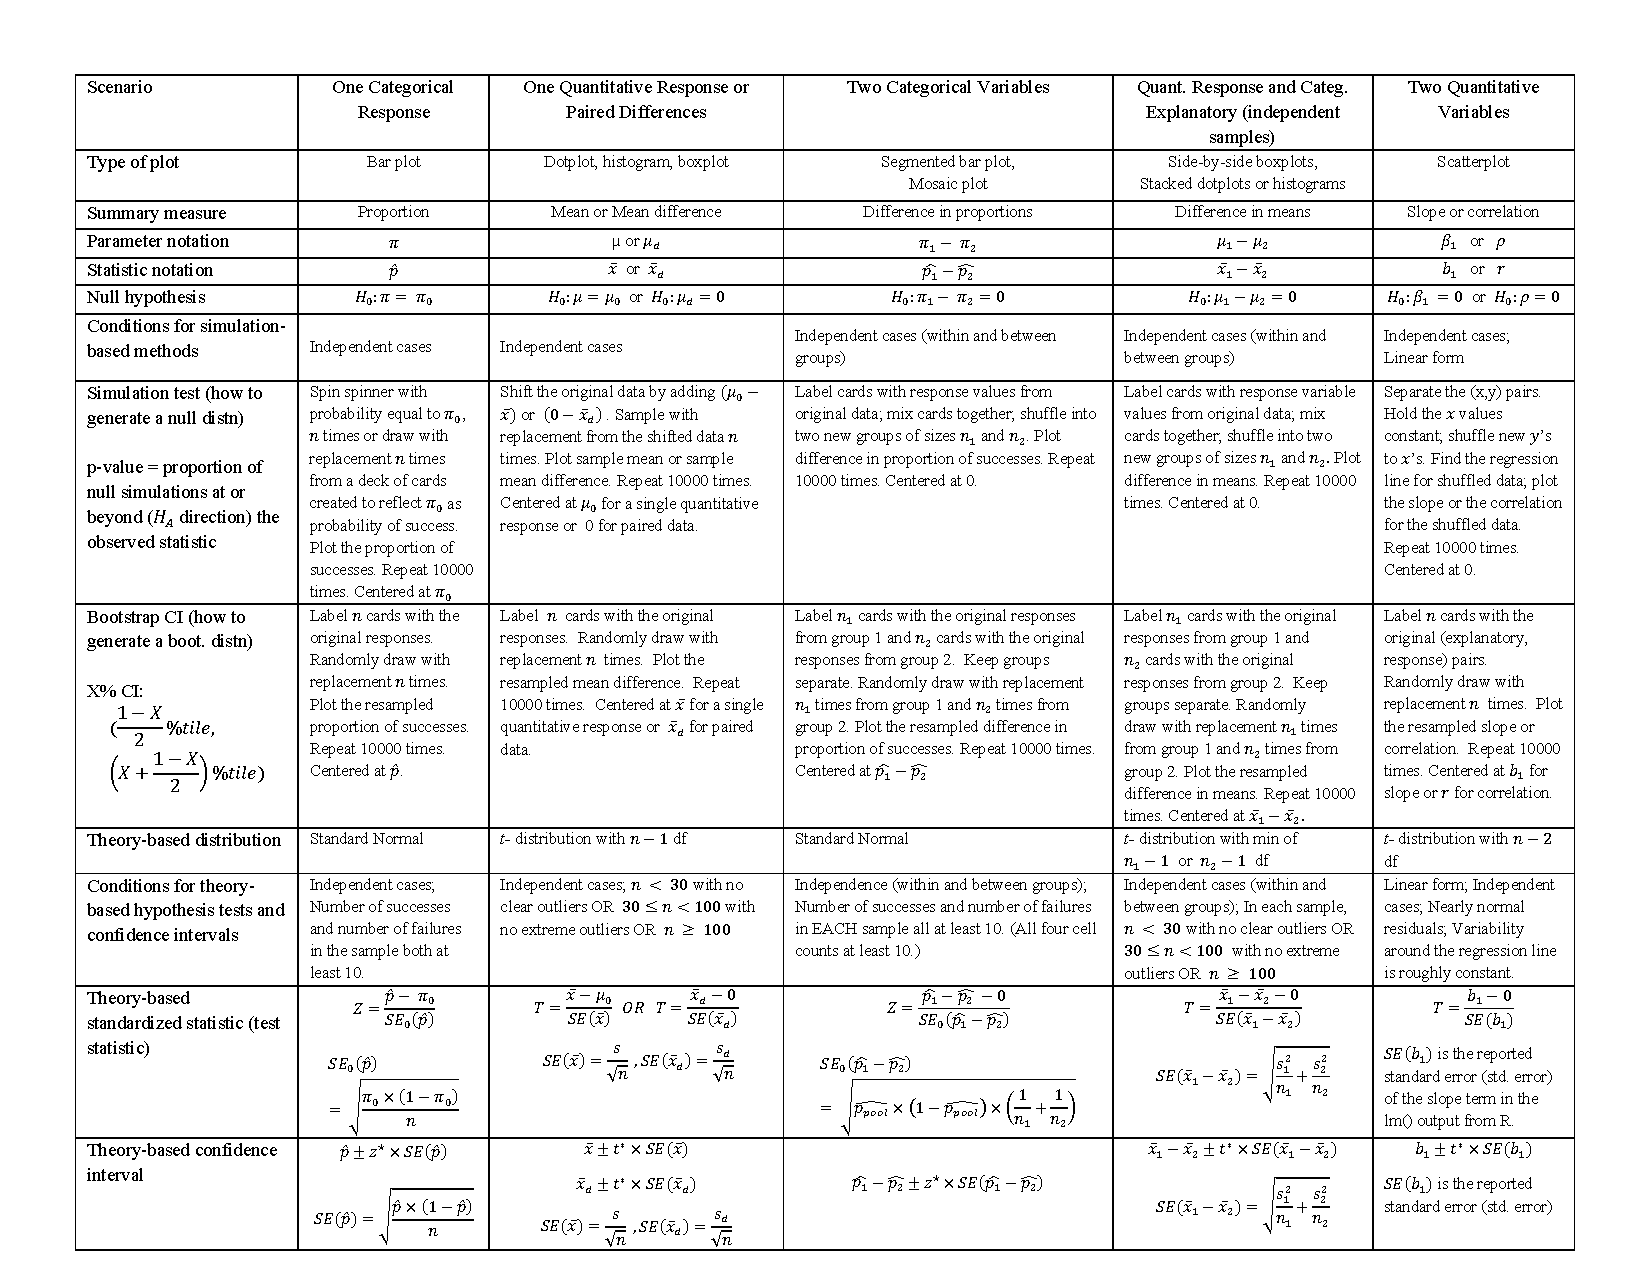
\includepdf[landscape=true]{GoldenTicket_S25.pdf}

\chapter*{References}\label{references}
\addcontentsline{toc}{chapter}{References}

\phantomsection\label{refs}
\begin{CSLReferences}{1}{0}
\bibitem[\citeproctext]{ref-pga}
{``Average Driving Distance and Fairway Accuracy.''} 2008. \href{https://www.pga.com/\%20and\%20https://www.lpga.com/}{https://www.pga.com/ and https://www.lpga.com/}.

\bibitem[\citeproctext]{ref-banton2022}
Banton, et al, S. 2022. {``Jog with Your Dog: Dog Owner Exercise Routines Predict Dog Exercise Routines and Perception of Ideal Body Weight.''} \emph{PLoS ONE} 17(8).

\bibitem[\citeproctext]{ref-bhavsar2022}
Bhavsar, et al, A. 2022. {``Increased Risk of Herpes Zoster in Adults \(\geq\)50 Years Old Diagnosed with COVID-19 in the United States.''} \emph{Open Forum Infectious Diseases} 9(5).

\bibitem[\citeproctext]{ref-islands}
Bulmer, M. n.d. {``Islands in Schools Project.''} \url{https://sites.google.com/site/islandsinschoolsprojectwebsite/home}.

\bibitem[\citeproctext]{ref-bts}
{``Bureau of Transportation Statistics.''} 2019. \url{https://www.bts.gov/}.

\bibitem[\citeproctext]{ref-babies}
{``Child Health and Development Studies.''} n.d. \url{https://www.chdstudies.org/}.

\bibitem[\citeproctext]{ref-darley1973}
Darley, J. M., and C. D. Batson. 1973. {``"From Jerusalem to Jericho": A Study of Situational and Dispositional Variables in Helping Behavior.''} \emph{Journal of Personality and Social Psychology} 27: 100--108.

\bibitem[\citeproctext]{ref-davis2020}
Davis, Smith, A. K. 2020. {``A Poor Substitute for the Real Thing: Captive-Reared Monarch Butterflies Are Weaker, Paler and Have Less Elongated Wings Than Wild Migrants.''} \emph{Biology Letters} 16.

\bibitem[\citeproctext]{ref-doit2015}
Du Toit, et al, G. 2015. {``Randomized Trial of Peanut Consumption in Infants at Risk for Peanut Allergy.''} \emph{New England Journal of Medicine} 372.

\bibitem[\citeproctext]{ref-edmunds2016}
Edmunds, et al, D. 2016. {``Chronic Wasting Disease Drives Population Decline of White-Tailed Deer.''} \emph{PLoS ONE} 11(8).

\bibitem[\citeproctext]{ref-ipeds}
Education Statistics, National Center for. 2018. {``IPEDS.''} \url{https://nces.ed.gov/ipeds/}.

\bibitem[\citeproctext]{ref-gbmarried}
{``Great Britain Married Couples: Great Britain Office of Population Census and Surveys.''} n.d. \url{https://discovery.nationalarchives.gov.uk/details/r/C13351}.

\bibitem[\citeproctext]{ref-zeitler2012}
Group, TODAY Study. 2012. {``\href{https://www.ncbi.nlm.nih.gov/pubmed/22540912}{A Clinical Trial to Maintain Glycemic Control in Youth with Type 2 Diabetes}.''} \emph{New England Journal of Medicine} 366: 2247--56.

\bibitem[\citeproctext]{ref-hamblin2007}
Hamblin, J. K., K. Wynn, and P. Bloom. 2007. {``Social Evaluation by Preverbal Infants.''} \emph{Nature} 450 (6288): 557--59.

\bibitem[\citeproctext]{ref-hirschfelder2018}
Hirschfelder, A., and P. F. Molin. 2018. {``I Is for Ignoble: Stereotyping Native Americans.''} \href{Retrieved\%20from\%20https://www.ferris.edu/HTMLS/news/jimcrow/native/homepage.htm.}{Retrieved from https://www.ferris.edu/HTMLS/news/jimcrow/native/homepage.htm.}

\bibitem[\citeproctext]{ref-hutchison2013}
Hutchison, R. L., and M. A. Hirthler. 2013. {``\href{https://www.ncbi.nlm.nih.gov/pubmed/23932117}{Upper Extremity Injuies in Homer's Iliad}.''} \emph{Journal of Hand Surgery (American Volume)} 38: 1790--93.

\bibitem[\citeproctext]{ref-imdb}
{``{IMDb} Movies Extensive Dataset.''} 2016. \url{https://kaggle.com/stefanoleone992/imdb-extensive-dataset}.

\bibitem[\citeproctext]{ref-kalra2022}
Kalra, et al., Dl. 2022. {``Trustworthiness of Indian Youtubers.''} Kaggle. \url{https://doi.org/10.34740/KAGGLE/DSV/4426566}.

\bibitem[\citeproctext]{ref-keating2021}
Keating, D., N. Ahmed, F. Nirappil, Stanley-Becker I., and L. Bernstein. 2021. {``Coronavirus Infections Dropping Where People Are Vaccinated, Rising Where They Are Not, Post Analysis Finds.''} \emph{Washington Post}. \url{https://www.washingtonpost.com/health/2021/06/14/covid-cases-vaccination-rates/}.

\bibitem[\citeproctext]{ref-laeng2007}
Laeng, Mathisen, B. 2007. {``Why Do Blue-Eyed Men Prefer Women with the Same Eye Color?''} \emph{Behavioral Ecology and Sociobiology} 61(3).

\bibitem[\citeproctext]{ref-levin2000}
Levin, D. T. 2000. {``Race as a Visual Feature: Using Visual Search and Perceptual Discrimination Tasks to Understand Face Categories and the Cross-Race Recognition Deficit.''} \emph{Journal of Experimental Psychology} 129(4).

\bibitem[\citeproctext]{ref-luetkemeier2017}
LUETKEMEIER, et al., M. 2017. {``Skin Tattoos Alter Sweat Rate and Na+ Concentration.''} \emph{Medicine and Science in Sports and Exercise} 49(7).

\bibitem[\citeproctext]{ref-madden2020}
Madden, et al, J. 2020. {``Ready Student One: Exploring the Predictors of Student Learning in Virtual Reality.''} \emph{PLoS ONE} 15(3).

\bibitem[\citeproctext]{ref-miller1956}
Miller, G. A. 1956. {``The Magical Number Seven, Plus or Minus Two: Some Limits on Our Capacity for Processing Information.''} \emph{Psychological Review} 63(2).

\bibitem[\citeproctext]{ref-becentispeech}
Moquin, W., and C. Van Doren. 1973. {``Great Documents in American Indian History.''} Praeger.

\bibitem[\citeproctext]{ref-pew2022}
{``More Americans Are Joining the 'Cashless' Economy.''} 2022. \url{https://www.pewresearch.org/short-reads/2022/10/05/more-americans-are-joining-the-cashless-economy/.}

\bibitem[\citeproctext]{ref-weather}
National Weather Service Corporate Image Web Team. n.d. {``National Weather Service -- {NWS} Billings.''} \url{https://w2.weather.gov/climate/xmacis.php?wfo=byz}.

\bibitem[\citeproctext]{ref-obrien2019}
O'Brien, Lynch, H. D. 2019. {``Crocodylian Head Width Allometry and Phylogenetic Prediction of Body Size in Extinct Crocodyliforms.''} \emph{Integrative Organismal Biology} 1.

\bibitem[\citeproctext]{ref-ocean}
{``Ocean Temperature and Salinity Study.''} n.d. \url{https://calcofi.org/}.

\bibitem[\citeproctext]{ref-WashPost2022}
{``Older People Who Get Covid Are at Increased Risk of Getting Shingles.''} 2022. \url{https://www.washingtonpost.com/health/2022/04/19/shingles-and-covid-over-50/.}

\bibitem[\citeproctext]{ref-physhealth}
{``Physician's Health Study.''} n.d. \url{https://phs.bwh.harvard.edu/}.

\bibitem[\citeproctext]{ref-porath2017}
Porath, Erez, C. 2017. {``Does Rudeness Really Matter? The Effects of Rudeness on Task Performance and Helpfulness.''} \emph{Academy of Management Journal} 50.

\bibitem[\citeproctext]{ref-quinn1999}
Quinn, G. E., C. H. Shin, M. G. Maguire, and R. A. Stone. 1999. {``Myopia and Ambient Lighting at Night.''} \emph{Nature} 399 (6732): 113--14. \url{https://doi.org/10.1038/20094}.

\bibitem[\citeproctext]{ref-ramachandran2007}
Ramachandran, V. 2007. {``3 Clues to Understanding Your Brain.''} \url{https://www.ted.com/talks/vs_ramachandran_3_clues_to_understanding_your_brain}.

\bibitem[\citeproctext]{ref-cdchospitalization}
{``Rates of Laboratory-Confimed COVID-19 Hospitalizations by Vaccination Status.''} 2021. CDC. \url{https://covid.cdc.gov/covid-data-tracker/\#covidnet-hospitalizations-vaccination}.

\bibitem[\citeproctext]{ref-richardson2019}
Richardson, T., and R. T. Gilman. 2019. {``Left-Handedness Is Associated with Greater Fighting Success in Humans.''} \emph{Scientific Reports} 9 (1): 15402. \url{https://doi.org/10.1038/s41598-019-51975-3}.

\bibitem[\citeproctext]{ref-stephens2020}
Stephens, R., and O. Robertson. 2020. {``Swearing as a Response to Pain: Assessing Hypoalgesic Effects of Novel "Swear" Words.''} \emph{Frontiers in Psychology} 11: 643--62.

\bibitem[\citeproctext]{ref-stewart2014}
Stewart, E. H., B. Davis, B. L. Clemans-Taylor, B. Littenberg, C. A. Estrada, and R. M. Centor. 2014. {``Rapid Antigen Group a Streptococcus Test to Diagnose Pharyngitis: A Systematic Review and Meta-Analysis''} 9 (11). \url{https://doi.org/10.1371/journal.pone.0111727}.

\bibitem[\citeproctext]{ref-stroop1935}
Stroop, J. R. 1935. {``Studies of Interference in Serial Verbal Reactions.''} \emph{Journal of Experimental Psychology} 18: 643--62.

\bibitem[\citeproctext]{ref-subach2022}
Subach, et al, A. 2022. {``Foraging Behaviour, Habitat Use and Population Size of the Desert Horned Viper in the Negev Desert.''} \emph{Soc.Open Sci} 9.

\bibitem[\citeproctext]{ref-sulheim2017}
Sulheim, S., A. Ekeland, I. Holme, and R. Bahr. 2017. {``Helmet Use and Risk of Head Injuries in Alpine Skiers and Snowboarders: Changes After an Interval of One Decade''} 51 (1): 44--50. \url{https://doi.org/10.1136/bjsports-2015-095798}.

\bibitem[\citeproctext]{ref-titanic}
{``Titanic.''} n.d. \url{http://www.encyclopedia-titanica.org}.

\bibitem[\citeproctext]{ref-covidvaccinetracker}
{``US COVID-19 Vaccine Tracker: See Your State's Progress.''} 2021. Mayo Clinic. \url{https://www.mayoclinic.org/coronavirus-covid-19/vaccine-tracker}.

\bibitem[\citeproctext]{ref-usepa2020}
US Environmental Protection Agency. n.d. {``Air Data -- Daily Air Quality Tracker.''} \url{https://www.epa.gov/outdoor-air-quality-data/air-data-daily-air-quality-tracker}.

\bibitem[\citeproctext]{ref-wahlstrom2014}
Wahlstrom, et al, K. 2014. {``Examining the Impact of Later School Start Times on the Health and Academic Performance of High School Students: A Multi-Site Study.''} \emph{Center for Applied Research and Educational Improvement}.

\bibitem[\citeproctext]{ref-watson2015}
Watson, et al., N. 2015. {``Recommended Amount of Sleep for a Heathy Adult: A Joint Consensus Statement of the American Academy of Sleep Medicine and Sleep Research Society.''} \emph{Sleep} 38(6).

\bibitem[\citeproctext]{ref-Weiss1988}
Weiss, R. D. 1988. {``Relapse to Cocaine Abuse After Initiating Desipramine Treatment.''} \emph{JAMA} 260(17).

\bibitem[\citeproctext]{ref-navajo2011}
{``Welcome to the Navajo Nation Government: Official Site of the Navajo Nation.''} 2011.\href{\%20Retrieved\%20from\%20https://www.navajo-nsn.gov/.}{Retrieved from https://www.navajo-nsn.gov/.}

\bibitem[\citeproctext]{ref-wilson2016}
Wilson, Woodruff, J. P. 2016. {``Vertebral Adaptations to Large Body Size in Theropod Dinosaurs.''} \emph{PLoS ONE} 11(7).

\end{CSLReferences}

\end{document}
